\section{Experiments}
\label{sec:experiments}

\subsection{Experimental setup}

The controlled environment isolates the two mechanisms that make state
conditioning valuable. It fixes a context budget of four and uses 16 candidates
in the redundancy study; the candidate-scaling study varies the pool size over
$K=4,8,16,32,64$ at a duplicate ratio of $.50$. Candidate value is generated
from a frozen subset-capable predictor, and Standalone Utility, the cached-only
router, and R-MUR use matched encoder and head capacity. All controlled results
are averaged over five independent runs. The standalone oracle ranks candidates
by the true standalone marginal and keeps that order fixed; the sequential
oracle recomputes the true marginal after every selection. The gap between
these two policies defines structural headroom.

Traffic forecasting provides a useful multi-context testbed because the
prediction at one sensor can draw on correlated neighbouring sensors, and
recent KBS models exploit increasingly rich spatiotemporal and cross-city
dependencies \citep{yang2025crosscity,yao2025shkd,zhou2025transformer,yan2026freqmamba}.
Our experiments do not introduce a forecasting backbone; the datasets are used
to evaluate context-selection policies under a common fixed predictor.

The real-data study uses six standard traffic benchmarks: METR-LA, PEMS-BAY,
PEMS03, PEMS04, PEMS07, and PEMS08. For each target sensor, a ridge predictor is fitted on
that target's training windows under a full, an empty, and a randomly masked
subset of its own candidate pool, and is then held fixed for candidate
evaluation, oracle computation, and router training; the predictor is
therefore specific to the target and is refitted for every target the protocol
evaluates. Candidate pools are constructed from the training segment with
history length 12, forecast horizon 12, 16 candidates, and a context budget of
four. The evaluation protocol fixes 32 evenly spaced target sensors per dataset
and repeats each target with three independent runs, giving 576 target-run
evaluations for the learned policies and 960 for the oracle policies. All
methods are evaluated on the same pools, and the learned methods share encoder
and head capacity. R-MUR uses a shortlist of four candidates, so a decision
evaluates the predictor on one quarter of the pool.

We report the prediction gain, that is, the loss reduction relative to the
anchor-only predictor; structural headroom $H_{\mathrm{state}}$; the
negative-transfer rate, that is, the fraction of evaluation episodes whose
routed loss exceeds the anchor-only loss; oracle recovery, that is, the ratio
of learned gain to sequential-oracle gain; and the number of predictor
evaluations per decision. Standalone Utility ranks candidates by a predicted
standalone marginal, and the cached-only router is the same state-conditioned
model without predictor-response features. Four further rules are evaluated on
the same episodes, candidate pools and frozen predictor, all of them
content-based and none of them trained or evaluating the predictor during
selection: facility location, which greedily maximises submodular coverage of
the candidate pool; the same rule with an added relevance term; greedy
determinantal point process selection, which maximises the log-determinant of a
similarity kernel; and $k$-center selection, which maximises the minimum
distance to the selected set. Differences across methods are reported with
hierarchical bootstrap intervals over 5000 replicates that resample targets
and then runs within a target, so both sources of variation enter the
interval.

\subsection{When does state conditioning matter?}

In the controlled redundancy study, structural headroom grows monotonically
with the duplicate ratio. At zero redundancy the standalone and sequential
oracles coincide, so a perfect standalone ranking loses nothing. As redundancy
increases, the gap reaches .286, and at duplicate ratios .50 and .75 the
learned router exceeds the standalone oracle even though that oracle uses the
true standalone utilities. Conditioning on the selected set therefore creates
decision value beyond what standalone scoring provides. The per-run ladder,
including the gains of both oracles, is reported in the supplementary material.

\begin{figure}[tbp]
  \centering
  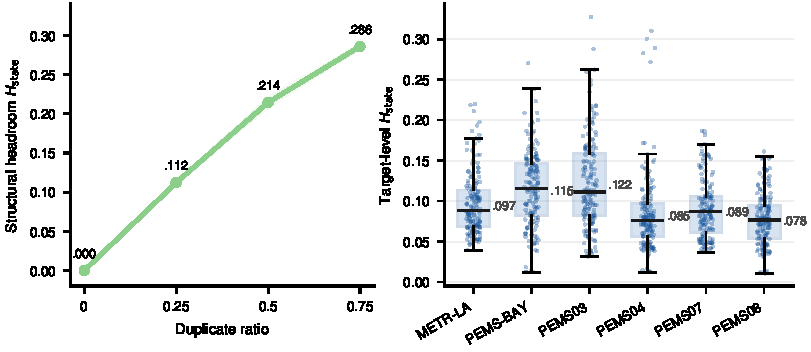
\includegraphics[width=0.98\linewidth]{figures/fig2_headroom.pdf}
  \caption{Structural headroom. Left: the gap between a perfect standalone
  ranking and a sequential oracle grows with the duplicate ratio, and the
  learned router exceeds the standalone oracle once redundancy is high. Right:
  target-level headroom on the six benchmarks, one point per target.}
  \label{fig:headroom}
\end{figure}

The same effect appears on real benchmarks. Over six datasets, 32 fixed targets
per dataset, and five independent runs, every one of the 960 target-run
evaluations has positive structural headroom. Figure~\ref{fig:headroom} shows
that the target-level distributions are concentrated rather than driven by a
few sensors: the per-dataset means range from .078 to .122 and the medians
from .076 to .116. Headroom of this size means that a router which only
reproduces a perfect standalone ranking leaves a measurable part of the
available loss reduction unused on every dataset and every target we evaluated.
Table~\ref{tab:headroom-real} reports the ratio together with the unnormalised
gap, which ranges from .005 to .019 in loss units.

% Generated by scripts/build_kbs_result_tables.py -- do not edit by hand.
% source: results/raw/R080a_multitarget_oracle_s5_*/<dataset>_s*/records.json
\begin{table}[t]
\centering
\small
\caption{Structural headroom per dataset over 32 fixed targets and
5 independent runs (960 target-run evaluations). The ratio and
the unnormalised difference are reported together; every evaluation has positive
headroom.}
\label{tab:headroom-real}
\resizebox{\linewidth}{!}{%
\begin{tabular}{lrrrr}
\toprule
Dataset & Mean $H_{\mathrm{state}}$ & Median $H_{\mathrm{state}}$ & Mean gap & Positive fraction\\
\midrule
METR-LA & .0966 & .0879 & .0143 & 1.000 \\
PEMS-BAY & .1153 & .1155 & .0188 & 1.000 \\
PEMS03 & .1221 & .1113 & .0071 & 1.000 \\
PEMS04 & .0848 & .0763 & .0052 & 1.000 \\
PEMS07 & .0891 & .0868 & .0057 & 1.000 \\
PEMS08 & .0778 & .0766 & .0050 & 1.000 \\
\bottomrule
\end{tabular}}
\end{table}


\subsection{Multi-target routing performance}

Table~\ref{tab:deployable} compares sixteen deployable selection policies
under the multi-target protocol. It contains the learned policies, which are
trained separately for each target-run on that target's training episodes;
four content-based rules that train nothing, namely facility location,
relevance-weighted facility location, greedy DPP, and $k$-center selection; and
five acquisition rules adapted from feature selection and active feature
acquisition, which choose one set per target on the validation split and then
apply it to every test episode. The fixed-set rules estimate how much of the
gain is available without conditioning a decision on the state of an individual
episode. Within a run all methods share the same candidate pool, the same fixed
predictor and the same evaluation episodes; the adaptation of each fixed-set
rule is described in the supplementary material. R-MUR obtains the best average
rank ($1.83$) and the lowest negative-transfer rate ($.335$) of the sixteen
methods compared, and it is the best response-free method on every dataset. It
is not the best method on every dataset, and we state where it is not: the
trivial policy of using all sixteen candidates exceeds it on PEMS04 ($+.0365$
against $+.0357$) and PEMS08 ($+.0359$ against $+.0333$), and the one-shot
response-aware variant exceeds it on PEMS04, PEMS07 and PEMS08. Paired against
pooling, under target-level paired intervals R-MUR is significantly ahead on
METR-LA ($+.0067$ $[+.0041,+.0094]$), PEMS-BAY ($+.0303$ $[+.0203,+.0427]$) and
PEMS07 ($+.0041$ $[+.0015,+.0070]$), is unresolved on PEMS03 ($+.0013$
$[-.0004,+.0030]$) and PEMS04 ($-.0008$ $[-.0050,+.0025]$), and is
significantly below on PEMS08 ($-.0026$ $[-.0042,-.0010]$). The strongest competitor on every benchmark is the
trivial policy of using every candidate, not any of the specialised subset
rules. The fixed-set rules are
the closest competitors on gain, and their harm rate is higher than that of
R-MUR even though they commit to a single set per target: tuning a set on
validation protects its average gain, not the individual episode, which is
again what per-episode conditioning provides. The content-based
rules that select by coverage or diversity alone, like relevance and maximum
marginal relevance, are negative on most datasets: covering the candidate pool
more evenly does not make the selected contexts more useful to the predictor.

The comparison forms a ladder in which each rung answers a different question.
Relevance, MMR, facility location, DPP and $k$-center all decide from cached
content alone, and their failure shows that neither similarity, nor diversity,
nor coverage is a reliable proxy for downstream predictive value. The fixed-set
rules are stronger than the content-based ones because they are tuned against
the predictor, and greedy validation selection is the closest competitor in the
table; it still remains below R-MUR on every dataset, so choosing the best set
offline is not a substitute for deciding per episode. That gap, small and
consistent, is the value that state conditioning adds. Standalone
Utility, which learns the value of a candidate in isolation, recovers part of
the gap but stays below the cached-only router on average, so a fixed candidate
value is not sufficient. The cached-only router conditions on the selected set
but never evaluates the predictor, and R-MUR improves on it on every dataset,
which isolates the contribution of the predictor response. The resulting order,
\[
\text{content-based rules}
\;<\;
\text{Standalone Utility}
\;\lesssim\;
\text{cached-only router}
\;<\;
\text{fixed-set acquisition}
\;<\;
\text{R-MUR},
\]
separates the four design decisions instead of reporting a single ranking:
choosing informative content, estimating a candidate's value, conditioning that
value on the selected set, and finally observing the predictor response.

% Generated by scripts/build_kbs_result_tables.py -- do not edit by hand.
% source: results/raw/R080b_multitarget_rmur_s*/<dataset>/target*_seed*/result.json
% source: results/raw/R202_subset_baselines_s3_*/<dataset>/target*_seed*/result.json
% source: results/raw/R206_fixed_set_baselines_v2_s3_*/<dataset>/target*_seed*/result.json
% source: results/raw/R207_oneshot_response_ablation_s3_*/<dataset>/target*_seed*/result.json
\begin{table}[t]
\centering
\small
\caption{Deployable selection methods under the multi-target protocol. Values are
prediction gains averaged over 32 fixed targets per dataset and over
3 independent runs. The first group holds the reference and learned
policies, the second content-based subset rules, and the third fixed-set
acquisition rules. The average rank is computed over all listed methods, and the
final column is the mean negative-transfer rate.}
\label{tab:deployable}
\resizebox{\linewidth}{!}{%
\begin{tabular}{lrrrrrrrr}
\toprule
Method & METR-LA & PEMS-BAY & PEMS03 & PEMS04 & PEMS07 & PEMS08 & Avg. rank & Neg. transfer\\
\midrule
Relevance & -.0165 & -.0199 & -.0191 & .0071 & -.0155 & .0074 & 15.17 & .5856\\
MMR & -.0180 & -.0249 & -.0102 & .0098 & -.0085 & .0075 & 14.67 & .5703\\
Standalone Utility & .0024 & .0272 & .0149 & .0248 & .0152 & .0246 & 7.00 & .4367\\
Cached-only router & .0042 & .0284 & .0154 & .0250 & .0150 & .0246 & 6.33 & .3944\\
R-MUR & .0146 & .0557 & .0269 & .0357 & .0284 & .0333 & 1.83 & .3346\\
Pool all 16 & .0080 & .0254 & .0256 & .0365 & .0242 & .0359 & 3.50 & .4270\\
Response-aware one-shot & -.0017 & .0502 & .0263 & .0382 & .0302 & .0353 & 2.67 & .4065\\
Facility location & -.0210 & .0077 & .0088 & .0139 & .0074 & .0171 & 10.17 & .4733\\
DPP greedy & -.0151 & .0053 & .0070 & .0131 & .0058 & .0120 & 10.33 & .4912\\
Facility location + relevance & -.0171 & -.0071 & -.0017 & .0123 & -.0023 & .0129 & 11.67 & .5321\\
k-center & -.0181 & -.0140 & .0044 & .0123 & .0031 & .0095 & 12.67 & .5168\\
Greedy validation set & .0088 & .0403 & .0197 & .0308 & .0182 & .0297 & 3.83 & .3850\\
Adaptive-$k$ relevance & -.0040 & -.0076 & -.0061 & .0087 & -.0052 & .0083 & 12.83 & .5559\\
Cluster-based selection & -.0162 & -.0127 & -.0055 & .0087 & -.0002 & .0125 & 12.50 & .5286\\
Two-step lookahead set & .0089 & .0402 & .0197 & .0308 & .0182 & .0297 & 4.17 & .3884\\
Gradient influence & .0004 & .0349 & .0131 & .0284 & .0144 & .0277 & 6.67 & .4157\\
\bottomrule
\end{tabular}}
\end{table}


\begin{figure}[tbp]
  \centering
  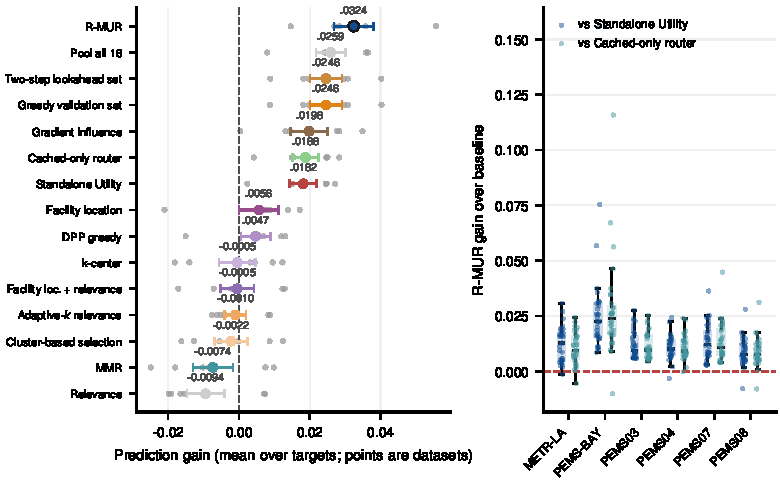
\includegraphics[width=0.98\linewidth]{figures/fig3_multitarget_delta.pdf}
  \caption{Multi-target comparison over fifteen deployable selection
  policies, including the trivial pool-everything policy that is the strongest
  competitor (the one-shot response ablation appears in
  Table~\ref{tab:deployable} only). Left: mean prediction gain across the six
  benchmarks, with the policies ordered by that mean; small points are the
  per-dataset target means and the interval is the standard error over
  datasets. Right: distribution over the 32 fixed targets of the R-MUR gain
  over Standalone Utility and over the cached-only router.}
  \label{fig:target-delta}
\end{figure}

Table~\ref{tab:consistency} reports the two contrasts that separate the
components of the method. The improvement over Standalone Utility shows that
state-conditioned marginal utility contains decision information that a fixed
candidate score does not; the improvement over the cached-only router shows
that evaluating the predictor on the shortlist adds information beyond a
state-conditioned score built from cached context features. Both differences
are positive on every dataset, and the hierarchical bootstrap intervals exclude
zero everywhere. The mean gain is positive on 81\% to 100\% of targets per
dataset, and 97\% to 100\% of targets exceed the standalone baseline, so the
improvement extends across prediction targets rather than being driven by a
single sensor. Oracle recovery ranges from .10 to .53. METR-LA shows the widest
target-level variation and the lowest recovery, while its dataset-level gain
remains positive.

% Generated by scripts/build_kbs_result_tables.py -- do not edit by hand.
% source: results/raw/R080b_multitarget_rmur_s*/<dataset>/target*_seed*/result.json
\begin{table}[t]
\centering
\small
\caption{Multi-target consistency of R-MUR over 32 fixed targets per dataset and
3 independent runs. Differences are computed per target and then
averaged; brackets are 95\% hierarchical bootstrap intervals that resample targets
and then runs within a target. Positive targets is
the fraction of targets whose mean gain is positive. Oracle recovery is the pooled
ratio of R-MUR gain to sequential-oracle gain.}
\label{tab:consistency}
\resizebox{\linewidth}{!}{%
\begin{tabular}{lrrrrrr}
\toprule
Dataset & $\Delta$ vs Static & $\Delta$ vs Cached & Positive targets & $>$ Static & $>$ Cached & Oracle recovery\\
\midrule
METR-LA & .0123 [.0082, .0168] & .0104 [.0069, .0142] & 0.812 & 0.969 & 0.969 & .099 \\
PEMS-BAY & .0285 [.0202, .0401] & .0272 [.0199, .0377] & 0.938 & 1.000 & 0.969 & .309 \\
PEMS03 & .0121 [.0099, .0145] & .0115 [.0095, .0136] & 1.000 & 1.000 & 1.000 & .447 \\
PEMS04 & .0109 [.0089, .0129] & .0107 [.0088, .0127] & 1.000 & 0.969 & 0.969 & .534 \\
PEMS07 & .0132 [.0104, .0161] & .0134 [.0105, .0167] & 1.000 & 1.000 & 1.000 & .456 \\
PEMS08 & .0088 [.0067, .0109] & .0087 [.0065, .0110] & 1.000 & 0.969 & 0.969 & .516 \\
\bottomrule
\end{tabular}}
\end{table}


Across the six benchmarks, R-MUR achieves the best average rank among all
sixteen evaluated deployable policies and is significantly ahead of the
strongest competitor on three of the six, unresolved on two and losing on one, so
these results establish it as the strongest *subset-selecting* method in our
unified evaluation of relevance-, diversity-,
coverage-, standalone-utility-, and state-conditioned selection. The two oracle policies serve as
structural references and are excluded from the deployable ranking: the
standalone oracle shows what a fixed ranking can reach, and the sequential
oracle what sequential information can reach.


\subsection{Why does R-MUR improve selection?}

Two mechanisms explain the result. The first is that larger candidate pools
compress the decision margin. In the controlled scaling study, the absolute
utility error improves as $K$ increases, but the standard deviation of the true
marginals falls faster: normalized error rises from .403 to .739, the positive
top-two margin falls from .220 to .024, and the median ratio of maximum
candidate error to that margin rises from 1.17 to 3.40. Selection accuracy
falls from .884 to .147, and one-step regret rises from .018 to .067 at $K=16$
and remains elevated at .049 at $K=64$. Pointwise regression error therefore
does not describe decision quality, which is why R-MUR is trained with a
gap-weighted ranking term in addition to regression.

The second mechanism is the information carried by the predictor response. With
cached context features only, the response-feature comparison reaches a
Spearman correlation of .164 and a positive-utility area under the receiver
operating characteristic curve of .649. Adding compact response summaries
raises them to .390 and .834, improves top-1 accuracy from .148 to .259, and
reduces one-step regret from .0736 to .0569. Full forecast trajectories add
little beyond the compact summaries. Figure~\ref{fig:mechanism} collects the
two mechanisms.

\begin{figure}[tbp]
  \centering
  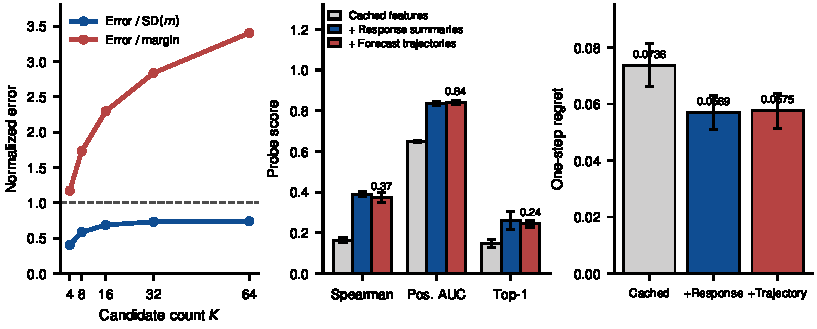
\includegraphics[width=0.98\linewidth]{figures/fig4_mechanism.pdf}
  \caption{Mechanisms. Left: as the candidate pool grows, the decision margin
  shrinks faster than the pointwise error, so selection accuracy falls.
  Middle: rank correlation, positive-utility AUC, and top-1 accuracy for
  cached features, compact response summaries, and full forecast trajectories.
  Right: one-step regret of the same three input sets.}
  \label{fig:mechanism}
\end{figure}

Table~\ref{tab:ablation} reports the component ablation under the multi-target
protocol. Using the whole pool without selection already improves over the
anchor, and it exceeds the cached-only router, which is state-conditioned but
never evaluates the predictor. R-MUR improves on both while evaluating the
predictor on a quarter of the pool and using about three contexts per episode.
The gap between the cached-only router and R-MUR is the contribution of the
predictor-response stage, and it is larger than the gap between the cached-only
router and a fixed standalone score.

% Generated by scripts/build_kbs_result_tables.py -- do not edit by hand.
% source: results/raw/R080b_multitarget_rmur_s*/<dataset>/target*_seed*/result.json
\begin{table}[t]
\centering
\small
\caption{Component ablation under the multi-target protocol, averaged over all
targets and runs of the primary multi-target evaluation, which comprises three
independent runs per target. Predictor evaluations is the share of the candidate
pool that receives a predictor evaluation per decision.}
\label{tab:ablation}
\resizebox{\linewidth}{!}{%
\begin{tabular}{lrrrr}
\toprule
Variant & Mean gain & Neg. transfer & Contexts used & Predictor evaluations\\
\midrule
Anchor only & .0000 & .0000 & .00 & 0 \\
Pool-all (no selection) & .0259 & .4270 & 16.00 & 100\% \\
Cached-only router & .0188 & .3944 & 3.18 & 0 \\
R-MUR & .0324 & .3346 & 3.05 & 25\% \\
\bottomrule
\end{tabular}}
\end{table}

\subsection{Routing budget and residual error}

Oracle recovery is between .10 and .53 (Table~\ref{tab:consistency}), so a
substantial part of the sequential-oracle gain is not realised. The regret
decomposition of Eq.~\eqref{eq:decomposition} locates it. At the deployed
shortlist size, the screening term accounts for 45\% to 55\% of the one-step
regret and the reranking term for the rest (Table~\ref{tab:decomposition}). The
loss is therefore not dominated by one stage: the cached screen misses the
truly best candidate often enough to matter, and the response-aware model
misranks the candidates it does see almost as often.

% Generated by scripts/build_shortlist_tables.py -- do not edit by hand.
% source: results/derived/R203_shortlist_diagnostics/summary.json (decomposition)
\begin{table}[t]
\centering
\small
\caption{One-step routing regret decomposed into the screening and reranking
terms of Eq.~\eqref{eq:decomposition}, in true marginal-utility units, at the
deployed shortlist size $q=4$. The final column is the screening share.}
\label{tab:decomposition}
\resizebox{\linewidth}{!}{%
\begin{tabular}{lrrrr}
\toprule
Dataset & Screening & Reranking & Total & Screening share\\
\midrule
METR-LA & .0319 & .0326 & .0645 & .49 \\
PEMS-BAY & .0298 & .0358 & .0656 & .45 \\
PEMS03 & .0083 & .0073 & .0156 & .53 \\
PEMS04 & .0080 & .0070 & .0151 & .53 \\
PEMS07 & .0092 & .0077 & .0169 & .55 \\
PEMS08 & .0077 & .0071 & .0149 & .52 \\
\bottomrule
\end{tabular}}
\end{table}


Table~\ref{tab:screening} shows how the screening term responds to the
shortlist size. Recall of the truly best candidate is .09--.12 at
$q=1$, .29--.33 at the deployed $q=4$, and .52--.57 at $q=8$, and the mean
screening regret falls from .020--.079 to .003--.017 over the same range.
Screening is thus the stage where additional predictor evaluations buy the most,
which is the quantitative version of the trade-off behind the shortlist: each
doubling of $q$ roughly doubles the probability that the best candidate is
available for reranking, at a proportional cost in predictor evaluations.

% Generated by scripts/build_shortlist_tables.py -- do not edit by hand.
% source: results/derived/R203_shortlist_diagnostics/summary.json (screening)
\begin{table}[t]
\centering
\small
\caption{Cached screening as a function of the shortlist size. Each cell reports
the recall of the truly best candidate and the mean screening regret in true
marginal-utility units.}
\label{tab:screening}
\resizebox{\linewidth}{!}{%
\begin{tabular}{lrrrrr}
\toprule
Dataset & $q=1$ & $q=2$ & $q=4$ & $q=8$ & $q=16$\\
\midrule
METR-LA & 0.09 / .070 & 0.17 / .048 & 0.29 / .032 & 0.52 / .017 & 1.00 / .000 \\
PEMS-BAY & 0.10 / .079 & 0.18 / .047 & 0.31 / .030 & 0.55 / .017 & 1.00 / .000 \\
PEMS03 & 0.10 / .021 & 0.17 / .013 & 0.30 / .008 & 0.55 / .004 & 1.00 / .000 \\
PEMS04 & 0.10 / .021 & 0.18 / .013 & 0.31 / .008 & 0.57 / .003 & 1.00 / .000 \\
PEMS07 & 0.10 / .024 & 0.17 / .015 & 0.30 / .009 & 0.54 / .004 & 1.00 / .000 \\
PEMS08 & 0.12 / .020 & 0.20 / .013 & 0.33 / .008 & 0.57 / .004 & 1.00 / .000 \\
\bottomrule
\end{tabular}}
\end{table}


\begin{figure}[tbp]
  \centering
  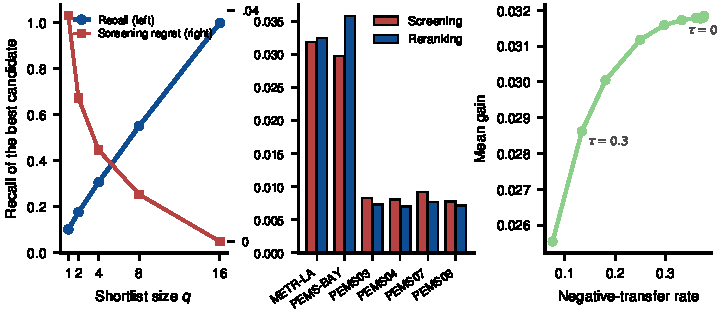
\includegraphics[width=0.98\linewidth]{figures/fig5_diagnostics.pdf}
  \caption{Shortlist diagnostics. Left: recall of the truly best candidate and
  screening regret as the shortlist grows. Middle: the one-step routing regret
  decomposed into its screening and reranking terms at the deployed shortlist
  size. Right: the gain--harm trade-off obtained by raising the stopping
  threshold.}
  \label{fig:diagnostics}
\end{figure}

The shortlist bounds the cost of a decision, and the stopping threshold decides how
much of it is used. At $q=4$ the predictor is evaluated on one quarter of the
pool, and Table~\ref{tab:screening} shows what that budget buys. The stopping
threshold is the second part of the cost, and it also controls how often
routing is harmful. Table~\ref{tab:calibration} sweeps the
threshold $\tau$ on the estimated marginal utility. At the deployed threshold
of zero the router keeps a mean gain of .0317 with a negative-transfer rate of
.332; raising the threshold to .3 keeps .0286 of the gain, reduces negative
transfer to .134 and uses about one context per episode; at .5 the router keeps
.0255 of the gain with a negative-transfer rate of .076.

The same table explains the residual negative transfer. At the deployed
threshold the positive-utility decision has precision .61 and recall .79: the
response-aware score identifies most useful candidates but over-predicts
usefulness, so a sign threshold is not a calibrated stopping rule. The sweep
exposes a clear operating trade-off between predictive gain and negative
transfer, and it turns the stopping rule into an explicit operating point
rather than a fixed constant. We report $\tau=0$ in all other results so that no
method is tuned on the evaluation targets.

% Generated by scripts/build_shortlist_tables.py -- do not edit by hand.
% source: results/derived/R203_shortlist_diagnostics/summary.json (threshold sweep)
\begin{table}[t]
\centering
\small
\caption{Stopping threshold sweep, averaged over the six datasets. Raising the threshold on the estimated marginal utility trades gain for a lower negative-transfer rate and fewer contexts. Coverage is the fraction of episodes on which the router selects at least one context. At the deployed threshold of zero the positive-utility decision has precision 0.61 and recall 0.79, where precision is the fraction of selected candidates with positive true marginal utility and recall is the fraction of positive-utility candidates that are selected.}
\label{tab:calibration}
\resizebox{\linewidth}{!}{%
\begin{tabular}{lrrrr}
\toprule
Threshold $\tau$ & Mean gain & Neg. transfer & Contexts & Coverage\\
\midrule
-0.40 & .0318 & .377 & 3.42 & 1.00 \\
-0.20 & .0318 & .375 & 3.40 & 1.00 \\
-0.10 & .0318 & .369 & 3.35 & 0.98 \\
-0.05 & .0318 & .360 & 3.28 & 0.97 \\
0.00 & .0317 & .332 & 3.05 & 0.91 \\
0.05 & .0316 & .298 & 2.44 & 0.84 \\
0.10 & .0312 & .250 & 1.93 & 0.74 \\
0.20 & .0300 & .181 & 1.34 & 0.58 \\
0.30 & .0286 & .134 & 0.98 & 0.47 \\
0.50 & .0255 & .076 & 0.56 & 0.32 \\
\bottomrule
\end{tabular}}
\end{table}


